%==============================================================
%  Figura 8.3 - Monitoraggio di posizione dei ripari mobili
%  mediante interruttori di prossimita' (Esempio 1)
%  Adattamento in italiano della Figura 8.3 dell'IFA Report 2/2017
%
%  I simboli riproducono quelli dell'originale: le coordinate sono
%  ricavate dal disegno di partenza (1 cm = 70 px, origine
%  nell'angolo in alto a sinistra della cornice).
%
%  NOTA: nel disegno compaiono simboli matematici ($<$, $\sim$):
%  niente cambi di corpo del font (font=\large & c.), che farebbero
%  fallire la composizione; le etichette sono ingrandite con "scale".
%==============================================================
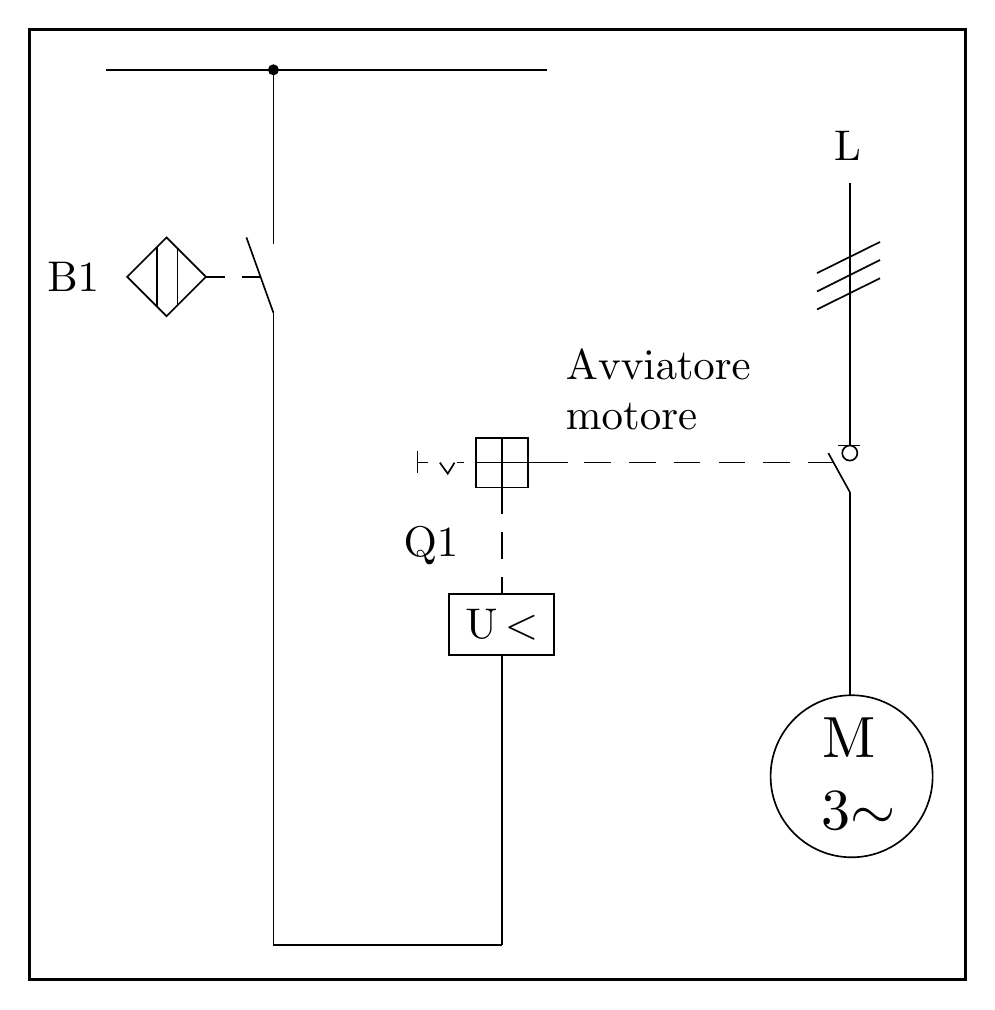
\begin{tikzpicture}[
  font=\normalsize,
  filo/.style={draw=black, line width=0.6pt},
  meccanico/.style={draw=black, line width=0.6pt, dash pattern=on 0.34cm off 0.23cm},
  etichetta/.style={inner sep=1pt, scale=1.55},
  grande/.style={inner sep=1pt, scale=2.1}
]

%--------------------------------------------------------------
% Cornice
%--------------------------------------------------------------
\draw[draw=black, line width=1.2pt] (0,0) rectangle (11.886,-12.071);

%--------------------------------------------------------------
% Linea di alimentazione del circuito di comando
%--------------------------------------------------------------
\draw[filo] (0.971,-0.514) -- (6.571,-0.514);
\fill[black] (3.10,-0.514) circle (0.07);

%--------------------------------------------------------------
% B1: interruttore di prossimita' con contatto di chiusura
%--------------------------------------------------------------
\draw[filo] (3.10,-0.514) -- (3.10,-2.729);
\draw[filo] (2.757,-2.643) -- (3.10,-3.60);
\draw[filo] (3.10,-3.60) -- (3.10,-11.629);
% collegamento di azionamento
\draw[filo] (2.243,-3.143) -- (2.486,-3.143);
\draw[filo] (2.700,-3.143) -- (2.936,-3.143);
% sensore
\draw[filo] (1.243,-3.143) -- (1.743,-2.643) -- (2.243,-3.143) -- (1.743,-3.643) -- cycle;
\draw[filo] (1.620,-2.766) -- (1.620,-3.520);
\draw[filo] (1.883,-2.783) -- (1.883,-3.503);
\node[etichetta] at (0.557,-3.143) {B1};

%--------------------------------------------------------------
% Q1: avviatore motore con sganciatore di minima tensione
%--------------------------------------------------------------
% organo di manovra con blocco meccanico
\draw[filo] (5.671,-5.186) rectangle (6.329,-5.820);
\draw[filo] (6.000,-5.186) -- (6.000,-5.820);
\draw[filo] (5.671,-5.503) -- (6.329,-5.503);
\draw[filo] (4.929,-5.357) -- (4.929,-5.629);
\draw[filo] (4.929,-5.503) -- (5.057,-5.503);
\draw[filo] (5.214,-5.503) -- (5.314,-5.643) -- (5.400,-5.503);
\draw[filo] (5.429,-5.503) -- (5.514,-5.503);
% collegamento meccanico verso il contatto principale
\draw[filo] (6.329,-5.503) -- (6.843,-5.503);
\draw[meccanico] (7.043,-5.503) -- (10.212,-5.503);
% collegamento meccanico verso lo sganciatore
\draw[meccanico] (6.000,-5.820) -- (6.000,-7.171);
% sganciatore di minima tensione
\draw[filo] (5.329,-7.171) rectangle (6.666,-7.943);
\node[etichetta] at (6.000,-7.557) {U\,$<$};
\draw[filo] (6.000,-7.943) -- (6.000,-11.629);
\draw[filo] (3.10,-11.629) -- (6.000,-11.629);
\node[etichetta] at (5.10,-6.557) {Q1};

%--------------------------------------------------------------
% Circuito di potenza: linea trifase L, contatto principale del
% Q1 e motore M
%--------------------------------------------------------------
\draw[filo] (10.42,-1.957) -- (10.42,-5.286);
\draw[filo] (10.004,-3.096) -- (10.804,-2.700);
\draw[filo] (10.004,-3.329) -- (10.804,-2.929);
\draw[filo] (10.004,-3.557) -- (10.804,-3.161);
\node[etichetta] at (10.39,-1.486) {L};
% contatto principale con apertura automatica
\draw[filo] (10.271,-5.286) -- (10.543,-5.286);
\draw[filo] (10.42,-5.381) circle (0.096);
\draw[filo] (10.147,-5.381) -- (10.42,-5.876);
\draw[filo] (10.42,-5.876) -- (10.42,-8.457);
% testo piu' lungo dell'originale inglese: allineato a sinistra ma
% spostato in modo da non toccare la linea L
\node[etichetta, anchor=base west] at (6.75,-4.45) {Avviatore};
\node[etichetta, anchor=base west] at (6.75,-5.08) {motore};
% motore trifase
\draw[filo] (10.443,-9.486) circle (1.029);
\node[grande] at (10.414,-9.00) {M};
\node[grande] at (10.53,-9.93) {3$\sim$};

\end{tikzpicture}
